% Corsin Week 2, transcript/week-02.md
\chapter{Week 2 --- Metric Spaces, Topology \& Continuity}

\exercisesheet{2}

\begin{notation}
No priority page this week: from Week 3 onwards Corsin opens each file with a colour-coded
\textit{Recommended exercises} page; Week 2 has none, so none of this week's problems are singled
out as important. The full sheet (2.1--2.7) is transcribed in
\texttt{content/exercise-sheets/week-02.tex}.
\end{notation}

\session{Monday}

\section{Structured spaces}
\label{sec:structured_spaces}

This semester you will be introduced to certain structures that can be given to a set --- also
called a \newterm{space} (\germanterm{Raum}) in this context --- which we will denote by $X$:

\begin{description}
  \item[0. Topological spaces] fourth semester.
  \item[1. Metric spaces] (\germanterm{metrischer Raum}) $(X,\ d : X \times X \to \mathbb{R}_{\geq 0})$
    \begin{itemize}
      \item Define a \textbf{distance} between points.
      \item $X$ is \textbf{not} necessarily a vector space.
      \item Covered in \textit{Analysis}.
    \end{itemize}
  \item[2. Normed metric spaces] $(X,\ \|\cdot\| : X \to \mathbb{R}_{\geq 0})$
    \begin{itemize}
      \item Define the \textbf{length} of a vector.
      \item Presuppose a linear structure, i.e.\ $X$ is a \textbf{vector space}.
      \item Covered in \textit{Linalg / Analysis}.
    \end{itemize}
  \item[3. Inner product spaces] $(X,\ \langle\cdot,\cdot\rangle : X \times X \to \mathbb{R})$
    \begin{itemize}
      \item Define \textbf{both} lengths \textbf{and} angles!
      \item Super important!
      \item Covered in \textit{Linalg}, sometimes used in \textit{Analysis}. $X$ is a vector space.
    \end{itemize}
\end{description}

\begin{center}
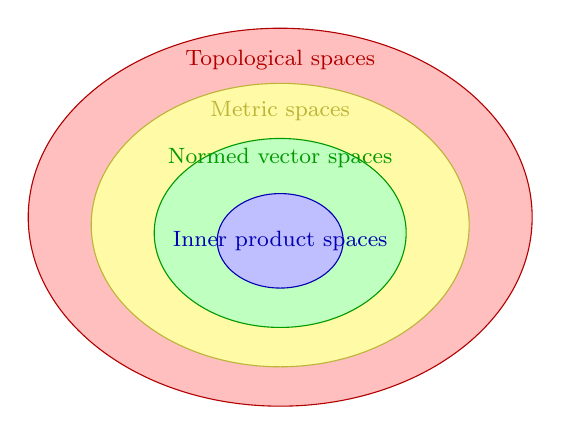
\begin{tikzpicture}
\fill[red!25] (0,0) ellipse (3.2 and 2.4);
\fill[yellow!35] (0,-0.1) ellipse (2.4 and 1.8);
\fill[green!25] (0,-0.2) ellipse (1.6 and 1.2);
\fill[blue!25] (0,-0.3) ellipse (0.8 and 0.6);
\draw[red!70!black] (0,0) ellipse (3.2 and 2.4);
\draw[yellow!70!black] (0,-0.1) ellipse (2.4 and 1.8);
\draw[green!60!black] (0,-0.2) ellipse (1.6 and 1.2);
\draw[blue!70!black] (0,-0.3) ellipse (0.8 and 0.6);
\node[red!70!black] at (0,2.0) {\footnotesize Topological spaces};
\node[yellow!70!black] at (0,1.35) {\footnotesize Metric spaces};
\node[green!60!black] at (0,0.75) {\footnotesize Normed vector spaces};
\node[blue!70!black] at (0,-0.3) {\footnotesize Inner product spaces};
\end{tikzpicture}
\end{center}

The precise definitions will follow later. You will see that an \textbf{inner product}
$\langle\cdot,\cdot\rangle$ induces a \textbf{norm} by the formula
$$\|x\| := \sqrt{\langle x, x\rangle}, \qquad x \in X.$$
Furthermore, a \textbf{norm} induces a \textbf{metric} by
$$d(x,y) := \|x - y\|, \qquad x, y \in X.$$

\section{Metric spaces}
\label{sec:metric_spaces}

\begin{definition}
\label{def:metric_space}
A \newterm{metric space} (\germanterm{metrischer Raum}) $(X,d)$ is any set $X$ with a
\newterm{metric} (\germanterm{Metrik}) $d : X \times X \to \mathbb{R}_{\geq 0}$ such that for all
$x, y, z \in X$:
\begin{description}
  \item[definiteness] $d(x,y) \geq 0$, with equality if and only if $x = y$. In words: the
    distance is non-negative, and a point has zero distance to itself.
  \item[symmetry] $d(x,y) = d(y,x)$, i.e.\ $x$ has the same distance to $y$ as $y$ to $x$.
  \item[triangle inequality] ($\Delta$-inequality) $d(x,z) \leq d(x,y) + d(y,z)$ ---
    \qt{detours make the way longer}.
\end{description}
\end{definition}

\begin{remark}
Corsin's gloss on definiteness reads \qt{the distance positive}; the formula $d \geq 0$ is
correct, but the gloss omits the ``non-''. Corrected in the prose above. See \texttt{OQ-02}.
\end{remark}

\begin{center}
\begin{tikzpicture}[>=Latex]
\draw[->] (-0.3,0) -- (4.2,0);
\draw[->] (0,-0.3) -- (0,3);
\coordinate (x) at (0.2,0.2);
\coordinate (y) at (1.6,2.0);
\coordinate (z) at (3.6,2.3);
\draw[blue,thick,->] (x) -- (y);
\draw[blue,thick,->] (y) -- (z);
\draw[red,thick,->] (x) -- (z);
\fill (x) circle (1.5pt) node[below]{$x$};
\fill (y) circle (1.5pt) node[above]{$y$};
\fill (z) circle (1.5pt) node[above]{$z$};
\node[red] at (2.3,0.7) {\footnotesize $d(x,z)$};
\node[blue] at (0.6,1.3) {\footnotesize $d(x,y)$};
\node[blue] at (2.7,2.4) {\footnotesize $d(y,z)$};
\node[red,below] at (2,-0.6) {\small $d(x,z) \le d(x,y)+d(y,z)$};
\end{tikzpicture}
\end{center}

\subsection{Examples}

\begin{example}
\label{ex:metric_examples}
\begin{enumerate}[label=\textbf{\arabic*.}]
  \item Let $X$ be a set. The \newterm{discrete metric} is given by
    $$d(x,y) = \begin{cases} 1 & \text{if } x \neq y \\ 0 & \text{if } x = y \end{cases}$$
    Important for counterexamples!
  \item Let $X = \mathbb{R}^n$. Then we have many choices for a metric; some common ones are:
  \begin{description}
    \item[(a) Manhattan metric:]
      $$d_1(x,y) = |x_1 - y_1| + \dots + |x_n - y_n| = \sum_{k=1}^{n} |x_k - y_k|$$
    \item[(b) Standard metric:]
      $$d_2(x,y) = \sqrt{(x_1-y_1)^2 + \dots + (x_n-y_n)^2} = \sqrt{\sum_{k=1}^{n}(x_k - y_k)^2}$$
    \item[(c) Supremum metric:]
      $$d_3(x,y) = \sup_{k = 1,\dots,n} |x_k - y_k|$$
  \end{description}
\end{enumerate}
\end{example}

\begin{figurestub}{FIG-W02-03}
Axes $x_1$ (horizontal), $x_2$ (vertical). Point $x = (x_1,x_2)$ lower-left, point
$y = (y_1,y_2)$ upper-right, each with dotted guide lines down/across to the axes. A right
triangle is formed: the blue hypotenuse runs diagonally from $x$ straight to $y$, labelled $d_2$;
the red vertical leg runs up the right side, at horizontal position $y_1$, from height $x_2$ to
$y$, labelled $d_1$; the orange horizontal leg runs along the bottom, at height $x_2$, from $x_1$
to $y_1$, labelled $d_3$.
\end{figurestub}

In general,
$$d(x,y) = \sqrt[m]{\sum_{k=1}^{n} (x_k - y_k)^m}$$
is a metric on $\mathbb{R}^n$ for any $m$.

\begin{example}[continued]
\begin{enumerate}[label=\textbf{\arabic*.}, start=3]
  \item $X = C^0([0,1], \mathbb{R})$, the set of continuous functions $[0,1] \to \mathbb{R}$.
    Then we can define the \textbf{supremum metric} for $f, g \in X$:
    $$d(f,g) = \sup_{x \in [0,1]} |f(x) - g(x)|$$
  \item $X = S^2 := \{(x_1,x_2,x_3) \in \mathbb{R}^3 : x_1^2 + x_2^2 + x_3^2 = 1\}$. $S^n$ is
    called the \textbf{$n$-dimensional sphere}, or \textbf{$n$-sphere}. The closest path between
    two points on the sphere is an \textbf{arc of a great circle} (a \textit{geodesic}). This
    defines a metric, similar to how straight lines define a metric on $\mathbb{R}^n$.
\end{enumerate}
\end{example}

\begin{figurestub}{FIG-W02-04}
Two panels, each a wireframe sphere (outline circle with a dashed equator ellipse for 3D
shading). Left panel: point $x$ red, near the front/bottom of the sphere; point $y$ red, near the
top; a blue arc runs over the surface between them, labelled $d(x,y)$. Right panel: the same
sphere outline with the same two points $x$ (lower) and $y$ (upper); the blue surface arc is
drawn again (labelled ``distance on sphere''), and in addition an orange dashed straight chord
cuts directly through the sphere's interior from $x$ to $y$ (labelled ``euclidean distance'').
\end{figurestub}

\begin{exercise}
\label{ex:sup_metric_is_metric}
Show that the supremum metric from \cref{ex:metric_examples}.3 is a metric.
\end{exercise}

\begin{exercisesolution}[\cref{ex:sup_metric_is_metric}]
Symmetry and definiteness are clear. For the triangle inequality, let $f, g, h \in C^0([0,1])$ and
set $p := f - h$, $q := h - g$. Then for all $x \in [0,1]$:
$$|p(x)| \leq \sup|p| \qquad \text{and} \qquad |q(x)| \leq \sup|q|.$$
Adding the inequalities, for all $x \in [0,1]$:
$$
\begin{aligned}
|f(x) - g(x)| = |p(x) + q(x)| &\leq |p(x)| + |q(x)| \\
&\leq \sup|p| + \sup|q| \\
&= \sup|f - h| + \sup|h - g|.
\end{aligned}
$$
\end{exercisesolution}

\section{Open and closed sets}
\label{sec:open_closed_sets}

\begin{definition}
\label{def:open_ball}
Let $(X,d)$ be a metric space, let $x \in X$, and let $r \in \mathbb{R}$. Then we define the
\newterm{open ball} of radius $r$ as
$$B_r(x) := \{\,\boxed{y \in X}\, : d(y,x) < r\,\}$$
\end{definition}

\begin{importantremark}
Corsin marks the boxed part in red as an \qt{important subtlety}: the ambient set $X$ in
$y \in X$ is what makes openness relative to the space, and it is exactly what the common
misconception on \cref{rem:common_misconception} turns on.
\end{importantremark}

\begin{remark}
\Cref{def:open_ball} is stated for $r \in \mathbb{R}$ rather than $r > 0$. Harmless here, but
loose. See \texttt{OQ-03}.
\end{remark}

\begin{definition}
Then we call a subset $U \subseteq X$ \newterm{open} (\germanterm{offen}) if and only if
$$\forall y \in U \ \exists \varepsilon > 0 \text{ such that } B_\varepsilon(y) \subseteq U.$$
And we call $A \subseteq X$ \newterm{closed} (\germanterm{abgeschlossen}) if and only if
$X \setminus A$ is open.
\end{definition}

\begin{exercise}
\label{ex:X_empty_clopen}
Let $(X,d)$ be a metric space. Show that $X$ and $\emptyset$ are both open and closed.
\end{exercise}

\begin{exercisesolution}[\cref{ex:X_empty_clopen}]
$X$ is open, since $B_r(x) \subseteq X$ for all $r > 0$, $x \in X$. The empty set contains no
points and is therefore vacuously open. Since $X$ and $\emptyset$ are each other's complement in
$X$, they are also closed.
\end{exercisesolution}

\subsection{Sequences and convergence}

\begin{definition}
A \newterm{sequence} $(x_n)_{n=0}^{\infty}$ in a metric space $(X,d)$ is a function
$x : \mathbb{N} \to X$. We say that $(x_n)_{n=0}^{\infty}$ \newterm{converges} to $x \in X$ if
$$\forall \varepsilon > 0 \ \exists N \in \mathbb{N} \text{ such that } d(x_n, x) < \varepsilon \quad \forall n \geq N.$$
\end{definition}

\begin{proposition}
\label{prop:open_closed_via_sequences}
\begin{enumerate}[label=\textbf{\arabic*.}]
  \item $U \subseteq X$ is \textbf{open} if and only if, for every sequence in $X$ with limit in
    $U$, the sequence eventually lies in $U$.
  \item $A \subseteq X$ is \textbf{closed} if and only if every convergent sequence in $A$ has its
    limit in $A$.
\end{enumerate}
\end{proposition}

\begin{example}[in $\mathbb{R}^2$]
In the euclidean metric space $\mathbb{R}^2$:
\begin{enumerate}[label=\textbf{\arabic*.}]
  \item $[0,1]^2$ is \textbf{closed}.
  \item $(0,1)^2$ is \textbf{open}.
  \item $[0,1] \times (0,1)$ is \textbf{neither open nor closed}.
\end{enumerate}
\end{example}

\begin{figurestub}{FIG-W02-05}
Three small square sketches side by side, one per case, each illustrating a converging sequence.
(1) $[0,1]^2$, closed --- solid-bordered square; a purple dotted trail labelled $x_n$ spirals
inward from the interior toward a red $\times$ marked at the top-right corner of the square (the
limit lies on the boundary, and belongs to the closed set). (2) $(0,1)^2$, open ---
dashed-bordered square; a purple dotted trail labelled $x_n$ approaches from just outside the
square's upper-left corner, illustrating a sequence whose limit (unmarked, on the boundary) would
not lie in the open set. (3) $[0,1]\times(0,1)$, neither --- square with solid left and right
edges but dashed top and bottom edges; an orange dotted trail labelled $y_n$ climbs toward a
point $y$ marked on the dashed top edge (limit not attained --- open side), while a purple dotted
trail labelled $x_n$ descends toward a red $\times$ at the bottom-right corner on a solid edge
(limit attained --- closed side).
\end{figurestub}

\begin{importantremark}[Common misconception!]
\label{rem:common_misconception}
In the euclidean metric space $X = [0,1]^2$, the set $[0,1]^2$ \textbf{is open}!
\begin{center}
\begin{tabular}{p{0.42\linewidth} p{0.42\linewidth}}
\textbf{$[0,1]^2 \subseteq \mathbb{R}^2$} & \textbf{$[0,1]^2 \subseteq [0,1]^2$} \\
Not open, since $B_\varepsilon(x)$ is not contained in $[0,1]^2$ if $x$ is on the boundary. &
Open, since the full space is always open, as shown before.
\end{tabular}
\end{center}
\end{importantremark}

\begin{figurestub}{FIG-W02-06}
Two square panels side by side, both depicting $[0,1]^2$. Left panel --- ambient space
$\mathbb{R}^2$: a red point $x$ sits on the square's boundary (right edge); an orange dashed
circle (the $\varepsilon$-ball centred at $x$) is drawn around it, extending visibly outside the
square's edge. Right panel --- ambient space $[0,1]^2$ itself: the same red boundary point $x$,
but the orange dashed $\varepsilon$-ball is clipped exactly at the square's edge, i.e.\ only the
portion of the disk lying inside the square is drawn.
\end{figurestub}

\begin{exercise}
\label{ex:uniform_convergence}
\begin{enumerate}[label=\textbf{\arabic*.}]
  \item Write down the definition of convergence of a sequence $(f_n)_{n=0}^{\infty}$ to $f$ in
    the metric space $X$ of bounded functions $[0,1] \to \mathbb{R}$ with the supremum metric.
  \item You know the resulting expression from Analysis 1. What is it called?
  \item \textit{(Optional)} Use the fact that $C^0([0,1]) \subseteq X$ is closed and
    \cref{prop:open_closed_via_sequences} on ``sequentially closed'' to conclude a big result
    from Analysis 1.
\end{enumerate}
\end{exercise}

\begin{exercisesolution}[\cref{ex:uniform_convergence}]
\begin{enumerate}[label=\textbf{\arabic*.}]
  \item $\displaystyle \forall \varepsilon > 0 \ \exists N \in \mathbb{N} : \sup_{x \in [0,1]} |f_n - f| < \varepsilon \quad \forall n \geq N$.
  \item This is \newterm{uniform convergence} (\germanterm{gleichm\"assige Konvergenz})!
  \item $C^0([0,1])$ is closed in the space of bounded functions with the supremum metric.

    \textit{Proof.} Let $f \in X \setminus C^0([0,1])$, i.e.\ $f : [0,1] \to \mathbb{R}$ is
    bounded and has at least one discontinuity at a point $x_0 \in [0,1]$. That is, we find
    $\varepsilon > 0$ such that for all $\delta > 0$ there exists $y \in (x_0 - \delta, x_0 +
    \delta)$ with $|f(x_0) - f(y)| \geq \varepsilon$. Then the $\tfrac{\varepsilon}{3}$-ball in
    $X$,
    $$B_{\varepsilon/3}(f) = \Big\{ g \in X : \sup_{x \in [0,1]} |f(x) - g(x)| < \tfrac{\varepsilon}{3} \Big\},$$
    is contained in $X \setminus C^0([0,1])$.

    Given this fact, \cref{prop:open_closed_via_sequences} ensures that the uniform limit $f$ of
    $(f_n)_{n=0}^{\infty}$ in $C^0([0,1])$ is also in $C^0([0,1])$, i.e.\ continuous, given that
    $f : [0,1] \to \mathbb{R}$ is bounded. This is the case, since $f_n$ is bounded for all
    $n \in \mathbb{N}$, and with $\varepsilon = 1$ we find $N \in \mathbb{N}$ such that
    $$\sup_{x \in [0,1]} |f_N(x) - f(x)| < 1 \implies f \text{ bounded.}$$
\end{enumerate}
\end{exercisesolution}

\begin{figurestub}{FIG-W02-07}
The ``$\varepsilon$-tube'': a blue curve $f$ on $[0,1]$ flanked by two red dotted curves at
vertical distance $\varepsilon/3$, with an orange double arrow marking $\varepsilon$. Caption:
$B_\varepsilon(f)$ in the space of bounded functions on $[0,1]$ is the ``$\varepsilon$-tube''
around $f$.
\end{figurestub}

\session{Friday}

\begin{warmup}
What is the shape of $B_1(0) \subseteq \mathbb{R}^2$ with the supremum metric? With the Manhattan
metric?
\end{warmup}

\begin{answer}
Supremum: the axis-aligned \textbf{square} $[-1,1]^2$, whose edge midpoints are $(\pm 1, 0)$ and
$(0,\pm 1)$. Manhattan: the \textbf{diamond} with vertices $(\pm 1, 0)$, $(0,\pm 1)$.
\end{answer}

\begin{figurestub}{FIG-W02-08}
Two axis systems side by side; left, a blue dashed square (supremum unit ball) with $(0,1)$ and
$(1,0)$ marked orange; right, a blue dashed diamond (Manhattan unit ball) with the same two
points marked.
\end{figurestub}

\section{Continuity}
\label{sec:continuity}

\begin{definition}
\label{def:continuous}
For $(X, d_X)$, $(Y, d_Y)$ metric spaces, a function $f : X \to Y$ is called \newterm{continuous}
(\germanterm{stetig}) if one of the following equivalent conditions holds:
\begin{enumerate}[label=\textbf{\arabic*.}]
  \item[\textbf{($\varepsilon$--$\delta$)}] $\forall x_0 \in X$, $\varepsilon > 0$
    $\exists \delta > 0$ such that for all $x \in X$:
    $$d(x_0, x) < \delta \implies d(f(x_0), f(x)) < \varepsilon$$
  \item[\textbf{(sequentially continuous)}] for any sequence $(x_n)_{n=0}^{\infty}$ in $X$ with
    limit $x \in X$, $\lim_{n\to\infty} f(x_n) = f(x)$ (and the limit exists).
  \item[\textbf{(topological)}] for all $U \subseteq Y$ open, $f^{-1}(U) \subseteq X$ is open.
\end{enumerate}
\end{definition}

\begin{remark}
Corsin writes $d(x_0,x) < \varepsilon$ in the ($\varepsilon$--$\delta$) hypothesis above, which
must read $\delta$ --- otherwise the quantified $\delta$ is never used. A slip of the pen;
corrected in \cref{def:continuous}. See \texttt{OQ-05}.
\end{remark}

\begin{example}
Let $f : \mathbb{R} \to \mathbb{R}$, $x \mapsto x^2$. Let $a < b \in \mathbb{R}$. Then
\begin{itemize}
  \item for $a < 0 < b$: $\quad f^{-1}((a,b)) = (-\sqrt{b}, \sqrt{b})$, open.
  \item for $a < b < 0$: $\quad f^{-1}((a,b)) = \emptyset$.
  \item for $0 < a < b$: $\quad f^{-1}((a,b)) = (-\sqrt{b}, -\sqrt{a}) \cup (\sqrt{a}, \sqrt{b})$.
\end{itemize}
\textit{Why is it enough to check only these cases?} Hint:
$f^{-1}(U_1 \cup U_2) = f^{-1}(U_1) \cup f^{-1}(U_2)$.
\end{example}

\begin{question}
Let $(X, d_X)$ and $(Y, d_Y)$ be metric spaces, where $d_Y$ is the discrete metric. Is
$f : (X,d_X) \to (Y,d_Y)$ continuous?
\end{question}

\begin{answer}
\textbf{No.} For example, take the spaces $X = Y = \mathbb{R}$, $d_X$ the standard metric, and
$f = \id : X \to Y$, $z \mapsto z$. Then $\{0\} \subseteq Y$ is open, but
$\{0\} = \id^{-1}\{0\}$ is not open in $(X, d_X)$.
\end{answer}

\begin{question}
What if $d_X$ is the discrete metric and $d_Y$ is arbitrary?
\end{question}

\begin{answer}
\textbf{Any} subset of $X$ is open; therefore $f^{-1}(U)$ is open for any open $U \subseteq Y$. So
every such $f$ is continuous.
\end{answer}

\section{Completeness}
\label{sec:completeness}

\begin{definition}
Let $(X,d)$ be a metric space and $(x_n)_{n=0}^{\infty}$ a sequence in $X$. We say that
$(x_n)_{n=0}^{\infty}$ is \newterm{Cauchy} if
$$\forall \varepsilon > 0 \ \exists N \in \mathbb{N} \text{ such that } d(x_n, x_m) < \varepsilon \quad \forall n, m \geq N.$$
$(X,d)$ is a \newterm{complete metric space} (\germanterm{vollst\"andiger metrischer Raum}) if
every Cauchy sequence in $X$ converges with respect to $d$.
\end{definition}

\begin{example}
\begin{itemize}
  \item The Euclidean spaces $(\mathbb{R}^n, \langle\cdot,\cdot\rangle_{\text{eucl}})$ are
    \textbf{complete}.
  \item Any \textbf{non-closed} subset $U \subseteq \mathbb{R}^n$ (standard metric) and the
    rationals $\mathbb{Q}$ are \textbf{not complete}.
  \item $\big(C^0([0,1]), \sup_{x \in [0,1]}|\cdot|\big)$ is \textbf{complete} (Zorich, p.\ 22).
\end{itemize}
\end{example}

\section{Compactness}
\label{sec:compactness}

\begin{definition}
A metric space $(X,d)$ is \newterm{compact} (\germanterm{kompakt}) if every open cover has a
finite subcover.
\end{definition}

\begin{theorem}
$(X,d)$ metric space is compact if and only if every sequence in $X$ has a convergent
subsequence in $X$.
\end{theorem}

\begin{figurestub}{FIG-W02-09}
A large blue freeform blob (cloud-like outline) labelled $X$. Inside it, three overlapping
dotted freeform loops, arranged Venn-style so every point of $X$ falls inside at least one:
$U_1$ (red) occupying roughly the lower area, $U_2$ (orange) occupying the upper-right, $U_3$
(purple) occupying the upper-left; all three overlap near the centre. Each label sits just
inside its own loop's boundary. Below, the annotation $U_1 \cup U_2 \cup U_3 = X$,
$U_i \subseteq X$ open sets.
\end{figurestub}

A subset $K$ of a metric space $(X,d)$ is compact if the metric space $(K, d|_{K \times K})$ is
compact. This is equivalent to the definition in the script:

\begin{definition}[9.63, quoted from the official lecture notes]
Let $(X,d)$ be a metric space. A subset $K \subset X$ is called \textbf{compact} if one of the
following equivalent conditions hold:
\begin{enumerate}[label=\textbf{\arabic*.}]
  \item $K$ is \textbf{sequentially compact}: every sequence $(x_n)_{n\in\mathbb{N}}$ in $K$ has
    a subsequence that is convergent in $K$.
  \item $K$ is \textbf{topologically compact}: every family of open sets $\{U_i\}_{i \in I}$ that
    cover $K$, has a finite subcover.
\end{enumerate}
\end{definition}

\begin{figurestub}{FIG-W02-10}
A large blue freeform blob labelled $X$, with a smaller purple/pink freeform blob $K$ nested
centrally inside it. Three dotted freeform loops overlap over $K$ and extend past its boundary
into the surrounding part of $X$ (but stay inside $X$): $U_1$ (green) lower-left, $U_2$ (orange)
upper, $U_3$ (magenta, dashed) right --- arranged so their union covers all of $K$. Below, the
annotation $K \subseteq U_1 \cup U_2 \cup U_3 \subseteq X$, $U_i \subseteq X$ open.
\end{figurestub}

\begin{exercise}
\label{ex:compact_finite_complete}
Let $(X,d)$ be a metric space.
\begin{enumerate}[label=\textbf{\arabic*.}]
  \item Show that every finite subset $\{x_1, \dots, x_n\} \subseteq X$ is compact.
  \item If $X$ is compact, is it complete?
\end{enumerate}
\end{exercise}

\begin{exercisesolution}[\cref{ex:compact_finite_complete}]
\begin{enumerate}[label=\textbf{\arabic*.}]
  \item Let $\{U_\alpha\}_{\alpha \in I}$ be an open cover of $\{x_1, \dots, x_n\}$. For each
    $i = 1, \dots, n$, pick $U_{\alpha_i}$ such that $x_i \in U_{\alpha_i}$. Then
    $\{U_{\alpha_i}\}_{i=1,\dots,n}$ is a finite subcover.
  \item \textbf{Yes.} Let $(x_n)_{n=0}^{\infty}$ be a Cauchy sequence in $X$. Then, because $X$ is
    compact, we find a convergent subsequence, $\lim_{i \to \infty} x_{n_i} = x \in X$.

    Fix $\varepsilon > 0$. We find $N_1 \in \mathbb{N}$ such that
    $$d(x_n, x_m) < \varepsilon \quad \forall n, m > N_1$$
    and $N_2 \in \mathbb{N}$ such that
    $$d(x, x_{n_i}) < \varepsilon \quad \forall i > N_2.$$
    For $N := \max\{N_1, N_2\}$ and $k > N$:
    $$d(x, x_k) \leq d(x, x_{n_k}) + d(x_{n_k}, x_k) < 2\varepsilon$$
    where we used $n_k \geq k > N$. So any Cauchy sequence converges.
\end{enumerate}
\end{exercisesolution}

\begin{remark}
Corsin writes $n_k > k$ above; for a subsequence the standing fact is $n_k \geq k$. Immaterial to
the argument. See \texttt{OQ-06}.
\end{remark}
